\documentclass{standalone}
\usepackage{tkz-graph}
\usetikzlibrary{arrows,positioning,shapes,shapes.multipart,patterns,mindmap,shadows}
\usepackage{xcolor}
\usepackage{helvet}
\renewcommand{\familydefault}{\sfdefault}


\begin{document}

\footnotesize
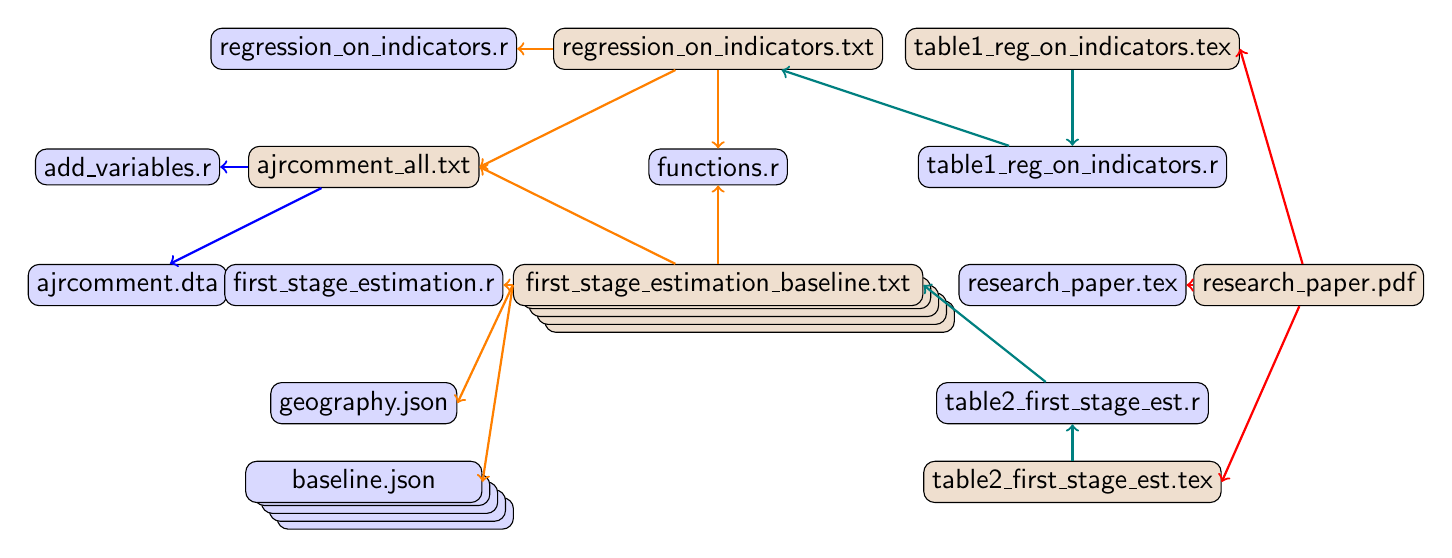
\begin{tikzpicture}[every node/.style={
    rectangle,
    rounded corners,
    inner sep=3pt,
    draw,
    fill=brown!25
}]
    \node (add_variables_r) [fill=blue!15, shift={(-4, 2)}]
    {
        add\_variables.r
    };
    \node (ajrcomment_dta) [fill=blue!15, shift={(-4, 0.5)}]
    {
        ajrcomment.dta
    };
    \node (ajrcomment_all_txt) [shift={(-1, 2)}]
    {
        ajrcomment\_all.txt
    };
    \node (first_stage_estimation_r) [fill=blue!15, shift={(-1, 0.5)}]
    {
        first\_stage\_estimation.r
    };
    \node (function_r) [fill=blue!15, shift={(3.5, 2)}]
    {
        functions.r
    };
    \node (regression_on_indicators_r) [fill=blue!15, shift={(-1, 3.5)}]
    {
        regression\_on\_indicators.r
    };
    \node (geography_json) [fill=blue!15, shift={(-1, -1)}]
    {
        geography.json
    };

    \node (newdata_json) [fill=blue!15, minimum width=3cm, minimum height=0.4cm, shift={(-0.6, -2.4)}] {};
    \node (rmconj_addindic_json) [fill=blue!15, minimum width=3cm, minimum height=0.4cm, shift={(-0.7, -2.3)}] {};
    \node (rmconj_json) [fill=blue!15, minimum width=3cm, minimum height=0.4cm, shift={(-0.8, -2.2)}] {};
    \node (addindic_json) [fill=blue!15, minimum width=3cm, minimum height=0.4cm, shift={(-0.9, -2.1)}] {};
    \node (baseline_json) [fill=blue!15, minimum width=3cm, minimum height=0.4cm, shift={(-1, -2)}]
    {
        baseline.json
    };



    \node (regression_on_indicators_txt) [shift={(3.5, 3.5)}]
    {
        regression\_on\_indicators.txt
    };


    \node (first_stage_estimation_newdata_txt) [minimum width=5.2cm, minimum height=0.4cm, shift={(3.9, 0.1)}] {};
    \node (first_stage_estimation_rmconj_addindic_txt) [minimum width=5.2cm, minimum height=0.4cm, shift={(3.8, 0.2)}] {};
    \node (first_stage_estimation_rmconj_txt) [minimum width=5.2cm, minimum height=0.4cm, shift={(3.7, 0.3)}] {};
    \node (first_stage_estimation_addindic_txt) [minimum width=5.2cm, minimum height=0.4cm, shift={(3.6, 0.4)}] {};
    \node (first_stage_estimation_baseline_txt) [minimum width=5.2cm, minimum height=0.4cm, shift={(3.5, 0.5)}]
    {
        first\_stage\_estimation\_baseline.txt
    };

    \node (research_paper_tex) [fill=blue!15, shift={(8, 0.5)}]
    {
        research\_paper.tex
    };
    \node (table2_first_stage_est_r) [fill=blue!15, shift={(8, -1)}]
    {
        table2\_first\_stage\_est.r
    };
    \node (table2_first_stage_est_tex) [shift={(8, -2)}]
    {
        table2\_first\_stage\_est.tex
    };
    \node (table1_reg_on_indicators_r) [fill=blue!15, shift={(8, 2)}]
    {
        table1\_reg\_on\_indicators.r
    };
    \node (table1_reg_on_indicators_tex) [shift={(8, 3.5)}]
    {
        table1\_reg\_on\_indicators.tex
    };
    \node (research_paper_pdf) [shift={(11, 0.5)}]
    {
        research\_paper.pdf
    };
    \draw[->, blue, thick] (ajrcomment_all_txt) to (add_variables_r);
    \draw[->, blue, thick] (ajrcomment_all_txt) to (ajrcomment_dta);
    \draw[->, orange, thick] (first_stage_estimation_baseline_txt) to (first_stage_estimation_r);
    \draw[->, orange, thick] (first_stage_estimation_baseline_txt.west) to (baseline_json.east);
    \draw[->, orange, thick] (first_stage_estimation_baseline_txt.west) to (geography_json.east);    
    \draw[->, orange, thick] (first_stage_estimation_baseline_txt) to (function_r);
    \draw[->, orange, thick] (first_stage_estimation_baseline_txt) to (ajrcomment_all_txt.east);
    \draw[->, orange, thick] (regression_on_indicators_txt) to (regression_on_indicators_r);
    \draw[->, orange, thick] (regression_on_indicators_txt) to (function_r);
    \draw[->, orange, thick] (regression_on_indicators_txt) to (ajrcomment_all_txt.east);
    
    \draw[->, teal, thick] (table1_reg_on_indicators_r) to (regression_on_indicators_txt);
    \draw[->, teal, thick] (table2_first_stage_est_r) to (first_stage_estimation_baseline_txt.east);
    \draw[->, teal, thick] (table1_reg_on_indicators_tex) to (table1_reg_on_indicators_r);
    \draw[->, teal, thick] (table2_first_stage_est_tex) to (table2_first_stage_est_r);

    \draw[->, red, thick] (research_paper_pdf) to (research_paper_tex.east);
    \draw[->, red, thick] (research_paper_pdf) to (table1_reg_on_indicators_tex.east);
    \draw[->, red, thick] (research_paper_pdf) to (table2_first_stage_est_tex.east);
\end{tikzpicture}

\end{document}